\documentclass{beamer}

\usepackage{float}
\usepackage{subfig}
\usepackage{graphicx}
\usepackage{changepage}
\graphicspath{{../figures/}}

%Information to be included in the title page:
\title{Exploration of Abalone game-playing agents}
\author{Ture Claussen}
\date{2021-06-14}


\begin{document}

\frame{\titlepage}

\begin{frame}
	\begin{figure}
		\frametitle{Rules}
		\centering
		\subfloat[Starting position]{
			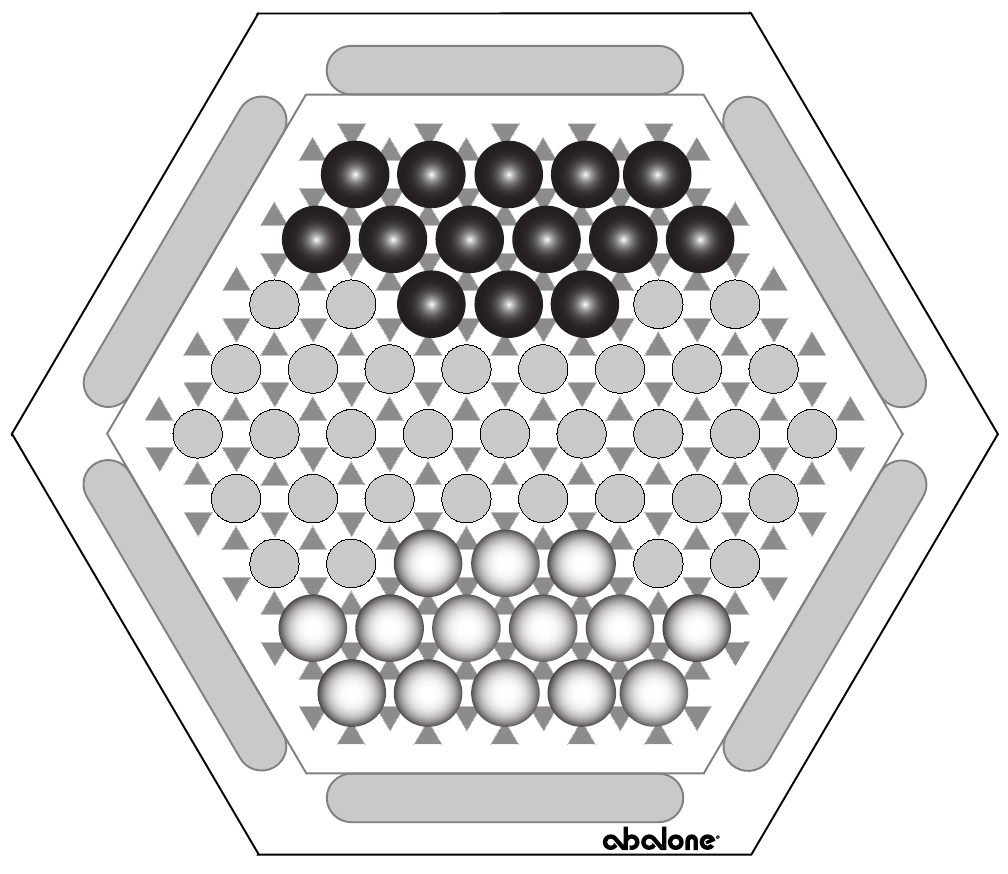
\includegraphics[width=3cm, keepaspectratio]{rules_starting_position.png}
		}
		\hfill
		\subfloat["In-line" moves]{
			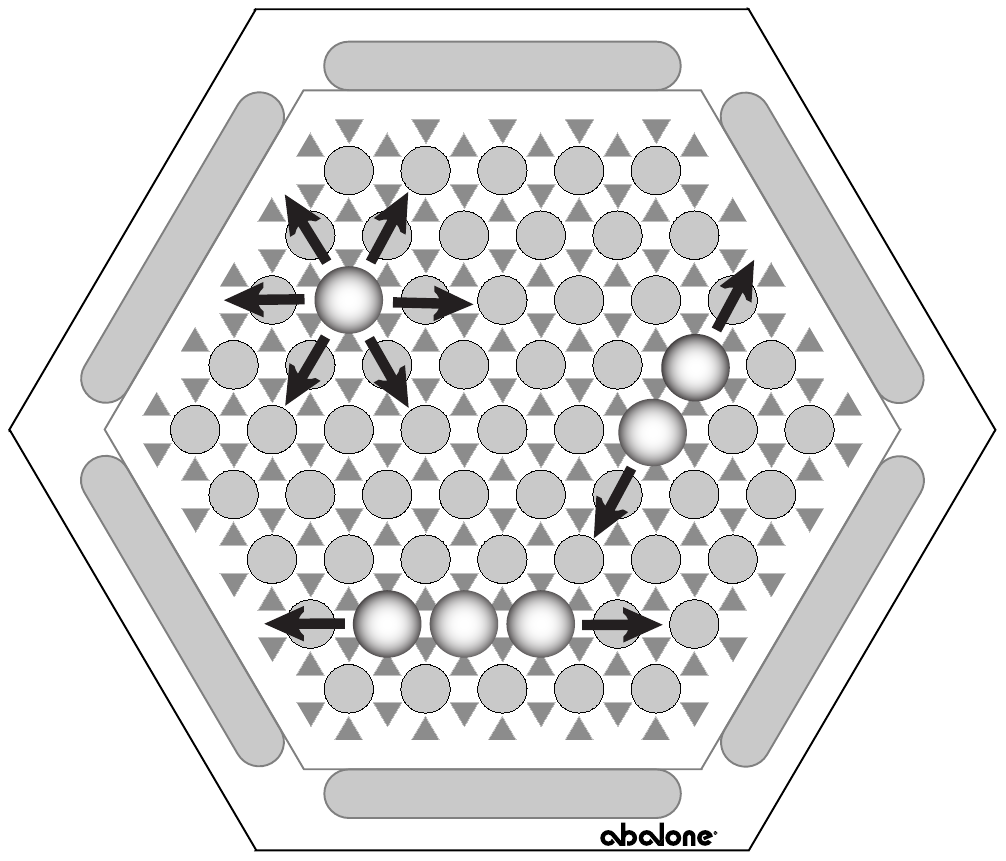
\includegraphics[width=3cm, keepaspectratio]{rules_inline_move.png}
		}
		\hfill
		\subfloat["Side-step" moves]{
			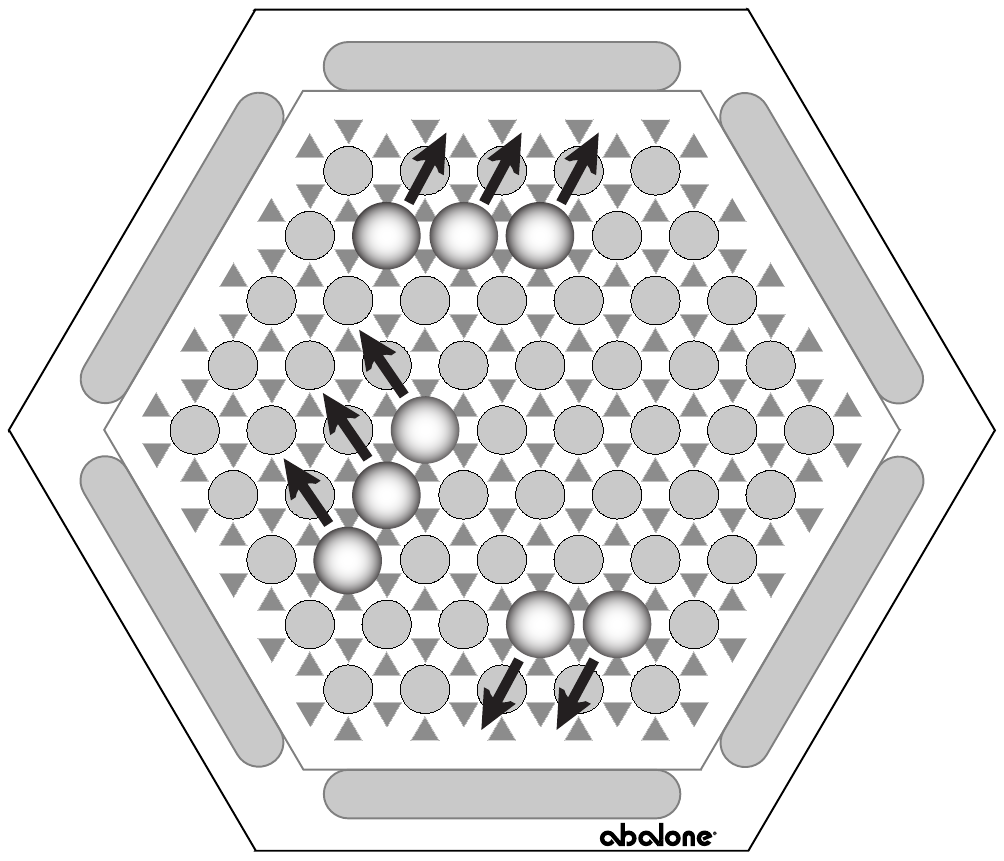
\includegraphics[width=3cm, keepaspectratio]{rules_side_step_move.png}
		}
	\end{figure}
\end{frame}

\begin{frame}

	\frametitle{Agent design: PEAS}

	\begin{description}
		\item[Performance measure] Win/loss, number of moves, time to deliberate
		\item[Environment] Digital playing board
		\item[Actuators] Move marbles, display text to CLI
		\item[Sensors] Position of marbles
	\end{description}
\end{frame}
\begin{frame}

	\frametitle{Agent design: Environment}

	\begin{itemize}
		\item fully observable
		\item two-agent
		\item competitive
		\item sequential
		\item static and discrete
	\end{itemize}
\end{frame}

\begin{frame}
	\frametitle{State space complexity}

	$$
		\sum_{k=8}^{14}\sum_{m=9}^{14}\frac{61!}{k!(61-k)!}\times\frac{(61-k)!}{m!((61-k)-m)!}
	$$
\end{frame}
\begin{frame}
	\frametitle{Game tree complexity}
	\begin{itemize}
		\item Average branching factor $b$ of 60
		\item Average length of game $d$ of 87 \cite{lemmens_constructing_2005}
	\end{itemize}
	$$ b^d = 60^{87}$$

	\begin{figure}
		\centering
		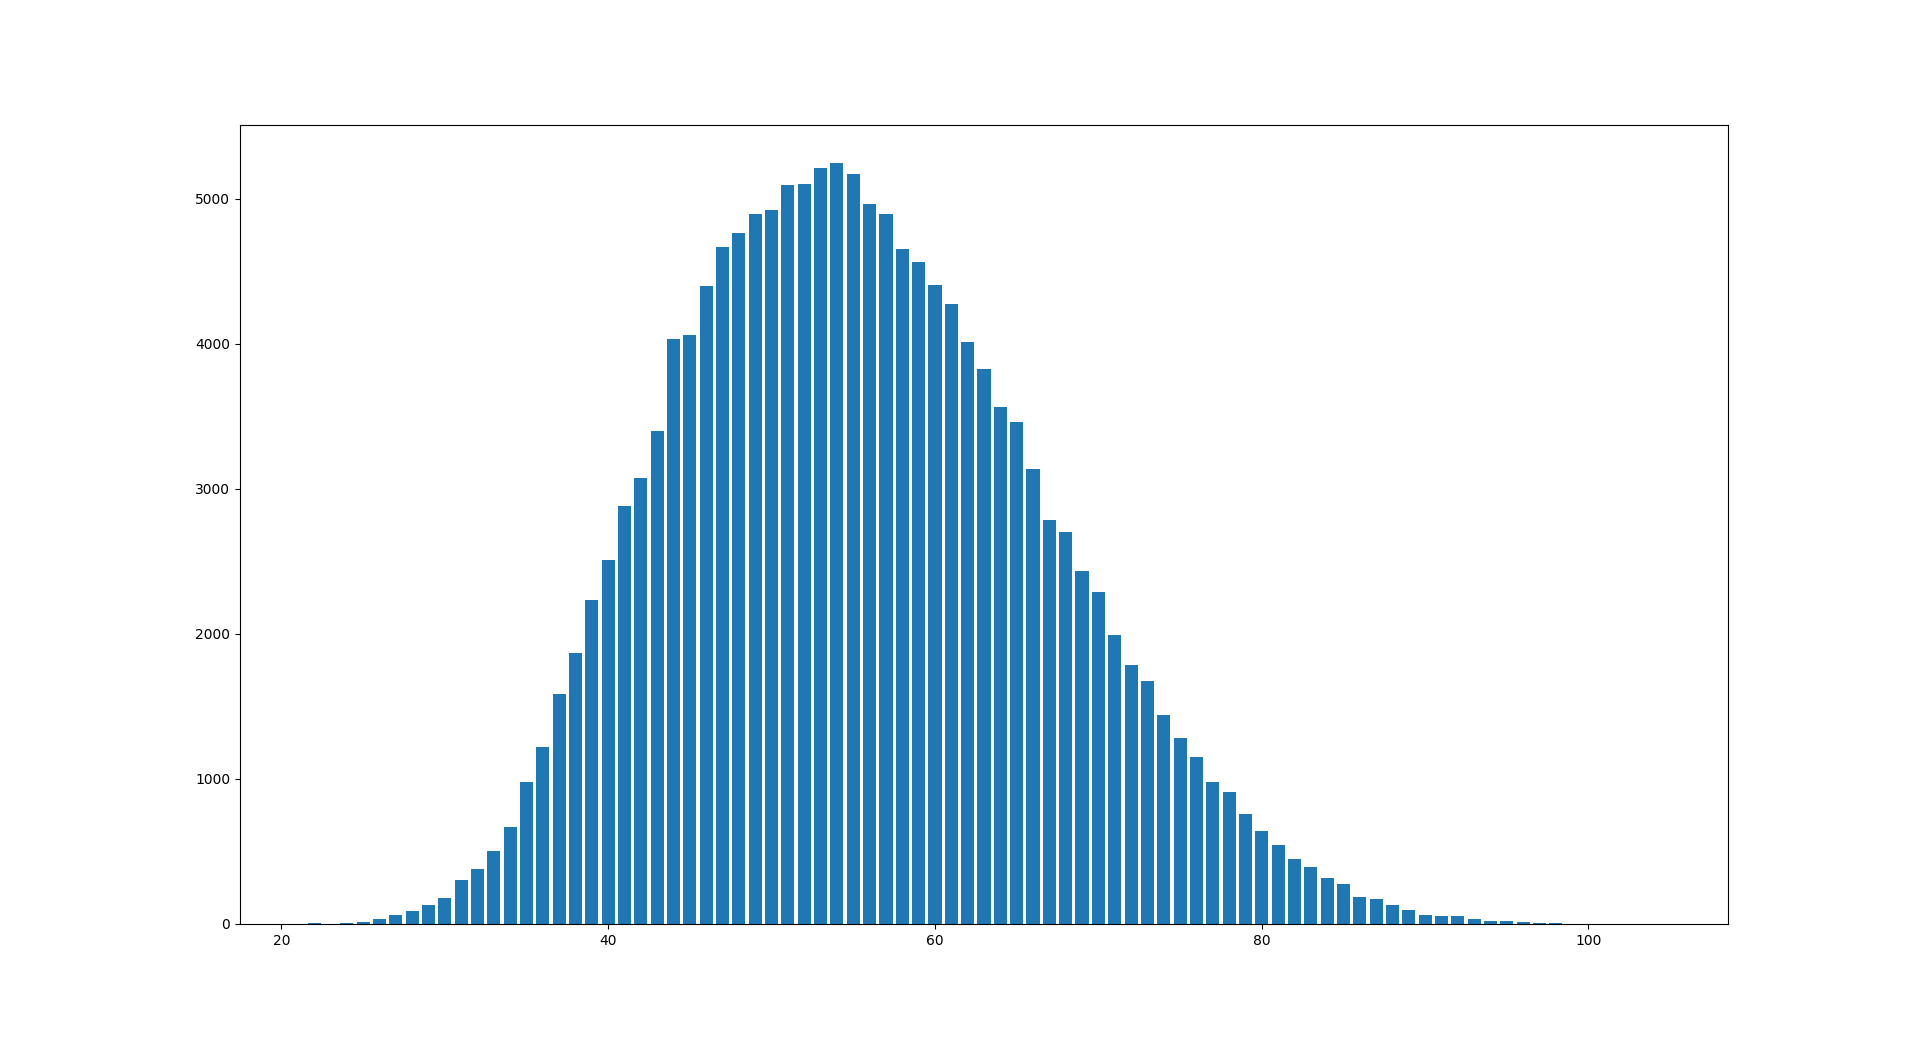
\includegraphics[width=7cm, keepaspectratio]{distribution_of_moves.png}
		\caption{Counts of moves available for random for random player in 5 games}
	\end{figure}
\end{frame}

\begin{frame}
	\frametitle{Complexity Comparision}
	\centering
	\begin{tabular}{ | c | c | c | }
		\hline
		Game        & \small{state-space complexity (log)} & \small{game-tree complexity} (log) \\
		\hline
		Tic-tac-toe & 3                                    & 5                                  \\
		\hline
		Reversi     & 28                                   & 58                                 \\
		\hline
		Chess       & 46                                   & 123                                \\
		\hline
		Abalone     & 24                                   & 154                                \\
		\hline
		Go          & 172                                  & 360                                \\
		\hline
	\end{tabular}
\end{frame}

\begin{frame}
	\frametitle{Heuristics: Ajdacency}
	\begin{figure}
		\centering
		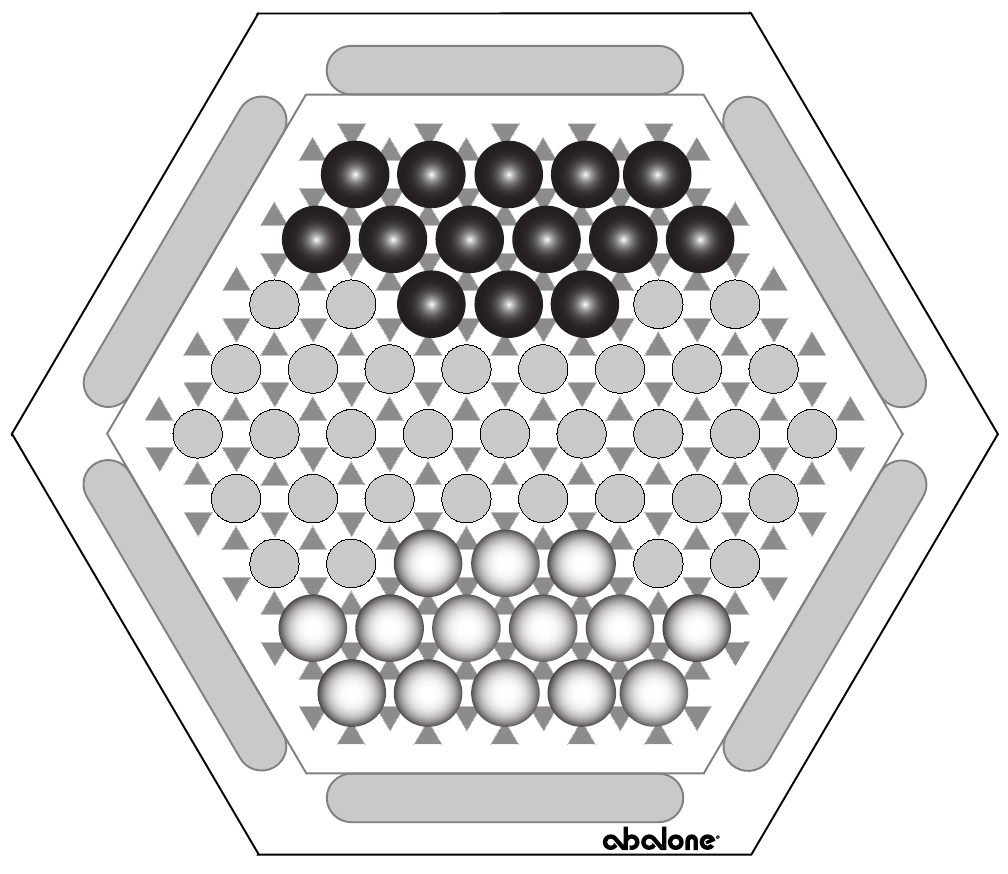
\includegraphics[width=5cm, keepaspectratio]{rules_starting_position.png}
	\end{figure}
	$$ \text{adjacency} = n_{\text{self}} - n_{\text{opponent}} $$
\end{frame}

\begin{frame}
	\frametitle{Heuristics: Distance}
	\begin{figure}
		\centering
		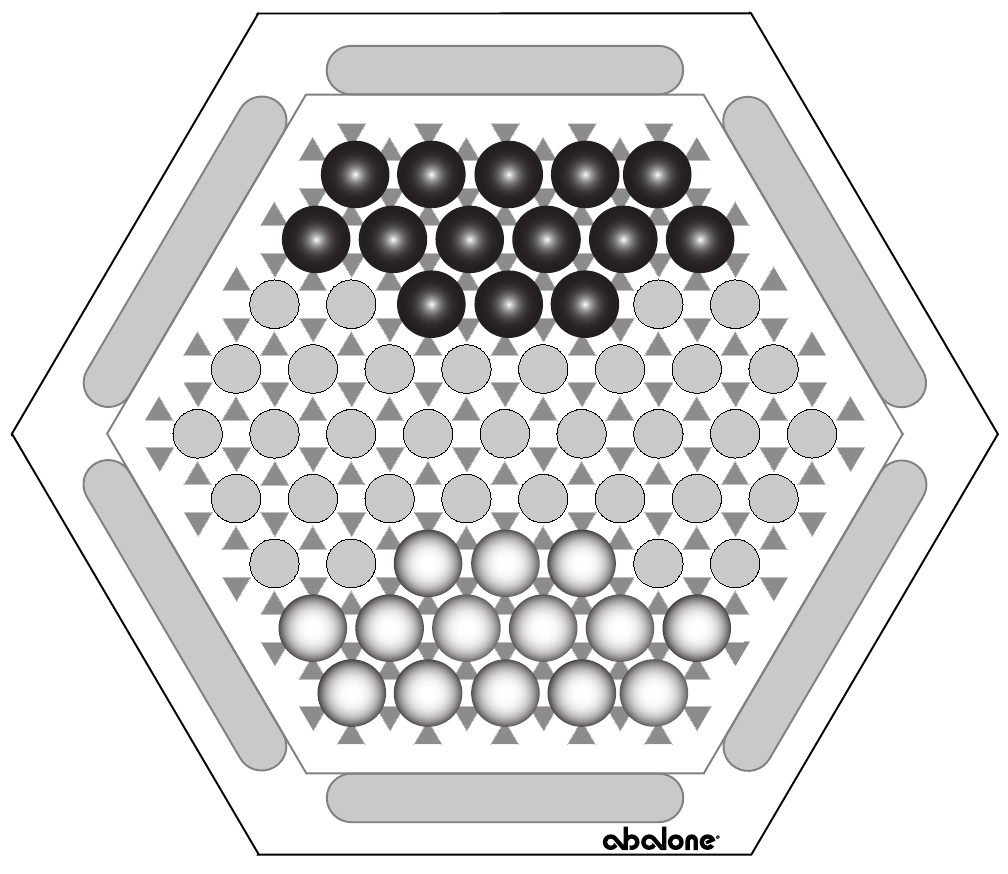
\includegraphics[width=5cm, keepaspectratio]{rules_starting_position.png}
	\end{figure}
	$$ \text{distance} = n_{\text{self}} - n_{\text{opponent}} $$
\end{frame}

\begin{frame}
	\frametitle{Heuristics: Marble ratio}
	$$ \text{marbleRatio} = n_{\text{won}} - n_{\text{lost}} $$

\end{frame}

\begin{frame}
	\frametitle{Heuristics: Win and loss}
	$$ \text{winLoss} =
		\begin{cases}
			1 \text{ if game won } \\
			-1 \text{ otherwise}
		\end{cases}
	$$

\end{frame}

\begin{frame}
	\begin{table}
		\begin{center}
			\begin{tabular}{ | c | c | }
				\hline
				Heuristic   & weight \\
				\hline
				adjacency   & 1      \\
				\hline
				distance    & -1.5   \\
				\hline
				marbleRatio & 100    \\
				\hline
				winLoss     & 100000 \\
				\hline
			\end{tabular}
		\end{center}
		\caption{Weights for the linear combination}
		\label{heuristic_table}
	\end{table}
\end{frame}

\begin{frame}
	\frametitle{Alpha-beta pruning agent: Move ordering}
	\begin{figure}
		\centering
		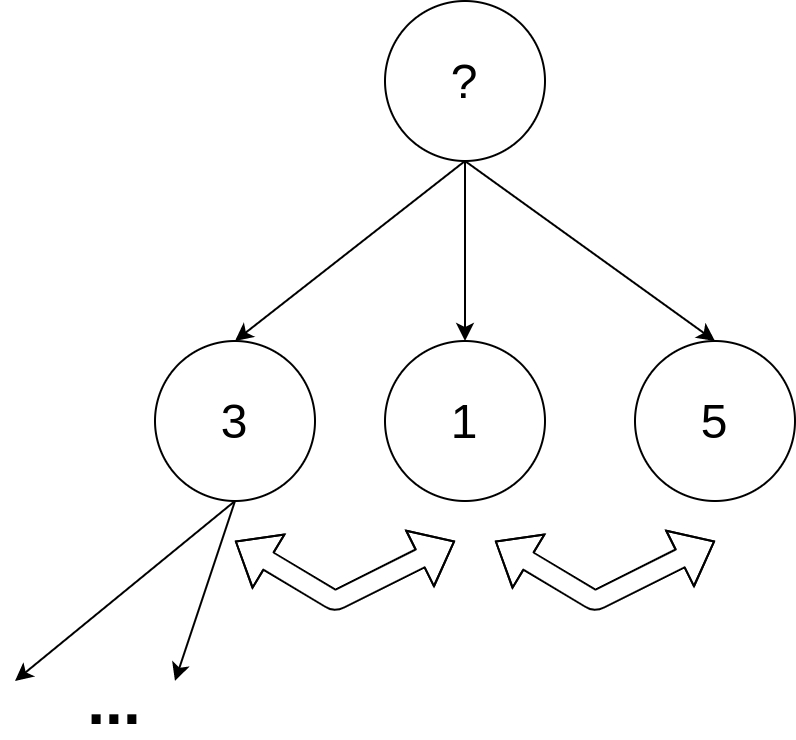
\includegraphics[width=7cm, keepaspectratio]{move_ordering.png}
	\end{figure}
\end{frame}

\begin{frame}
	\frametitle{Alpha-beta pruning agent: Move ordering}
	\begin{itemize}
		\item Move capturing marble: +3
		\item Move pushing marble: +1
		\item Move involving 2/3 marbles: +1/+2
	\end{itemize}
\end{frame}
\begin{frame}
	\frametitle{Alpha-beta pruning agent: Move ordering}
	\begin{table}
		\begin{center}
			\begin{tabular}{ | c | c | c | c | c | }
				\hline
				Depth & Without ordering & Evaluation 1 & Evaluation 2 & $\sqrt{b^d}$ \\
				\hline
				1     & 45               & 45           & 45           & 8            \\
				\hline
				2     & 1594             & 304          & 132          & 60           \\
				\hline
				3     & 9755             & 4971         & 2423         & 464          \\
				\hline
				4     & 457309           & 94650        & 6918         & 3600         \\
				\hline
			\end{tabular}
		\end{center}
		\caption{Nodes visited with/without move ordering and the optimal case}
		\label{node_count}
	\end{table}

\end{frame}

\begin{frame}
	\frametitle{Alpha-beta pruning agent: Transposition table}
	\begin{table}
		\begin{center}
			\begin{tabular}{ | c | c | c | c | }
				\hline
				    & 1            & 2            & ... \\
				\hline
				1   & 129310293812 & 929310293912 & ... \\
				\hline
				2   & 889394293012 & 426317297917 & ... \\
				\hline
				... & ...          & ...          & ... \\
				\hline
			\end{tabular}
		\end{center}
		\caption{Zobrist hash table}
		\label{heuristic_table}
	\end{table}

\end{frame}


\begin{frame}
	\frametitle{Alpha-beta pruning agent: Branch cutting}
	\begin{figure}
		\centering
		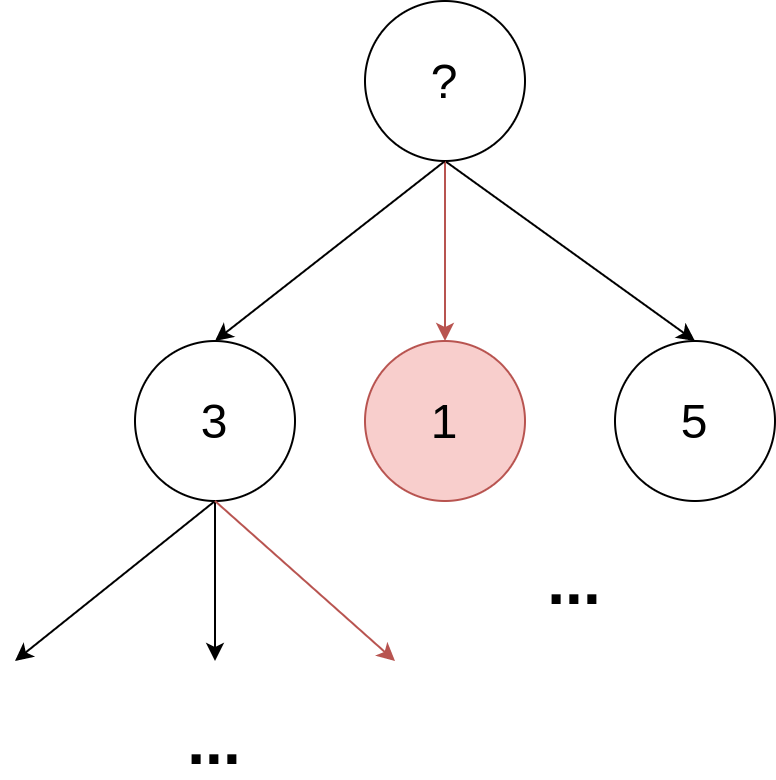
\includegraphics[width=7cm, keepaspectratio]{branch_cutting.png}
	\end{figure}
\end{frame}

\begin{frame}
	\frametitle{Monte carlo search agent}
	\begin{figure}
		\centering
		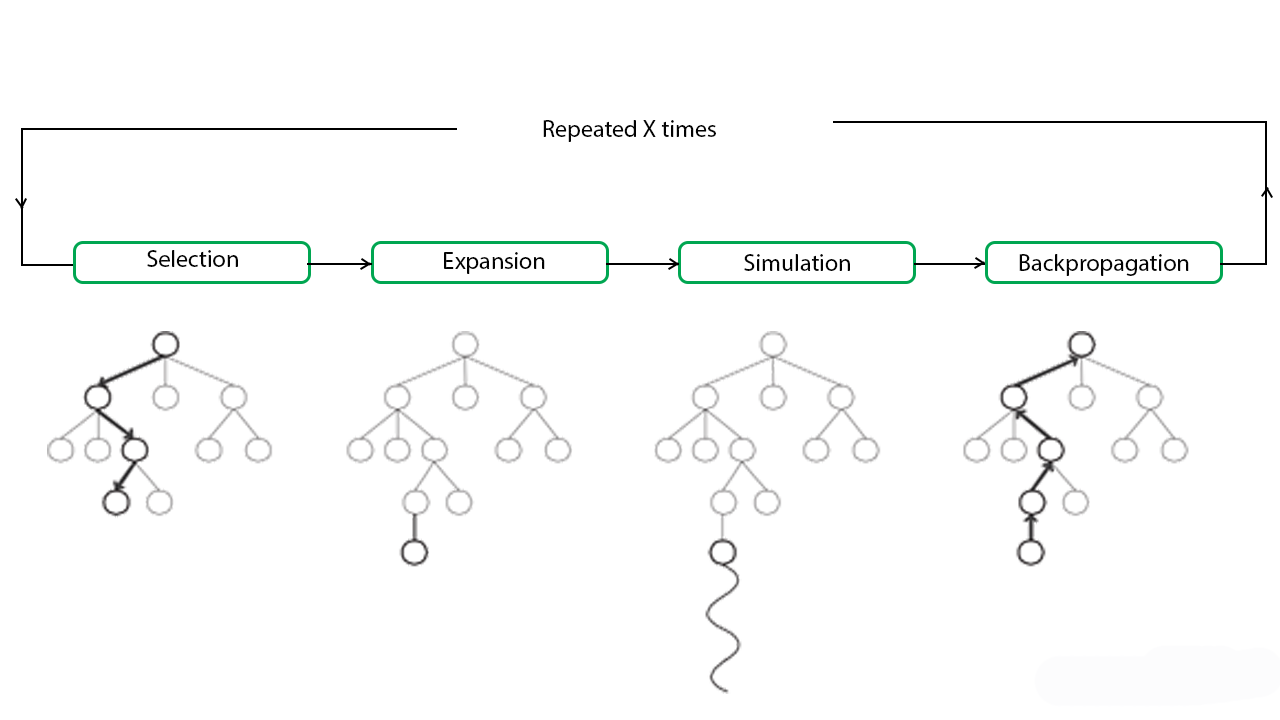
\includegraphics[width=10cm, keepaspectratio]{mcts_algo.png}
	\end{figure}
\end{frame}

\begin{frame}
	\frametitle{Monte carlo search agent: UCB}
	$$
		UCB(n) = \frac{U(n)}{N(n)} + C \times \sqrt{\frac{\log{N(Parent(n))}}{N(n)}}
	$$
\end{frame}
\begin{frame}
	\frametitle{Monte carlo search agent: Playout policy}
	\begin{itemize}
		\item Random moves bad as branching factor is high
		\item Choose moves based on evaluation function
	\end{itemize}
\end{frame}

\begin{frame}
	\frametitle{Face-off}
	\begin{adjustwidth}{-5in}{-5in}% adjust the L and R margins by 1 inch
		\begin{figure}
			\centering
			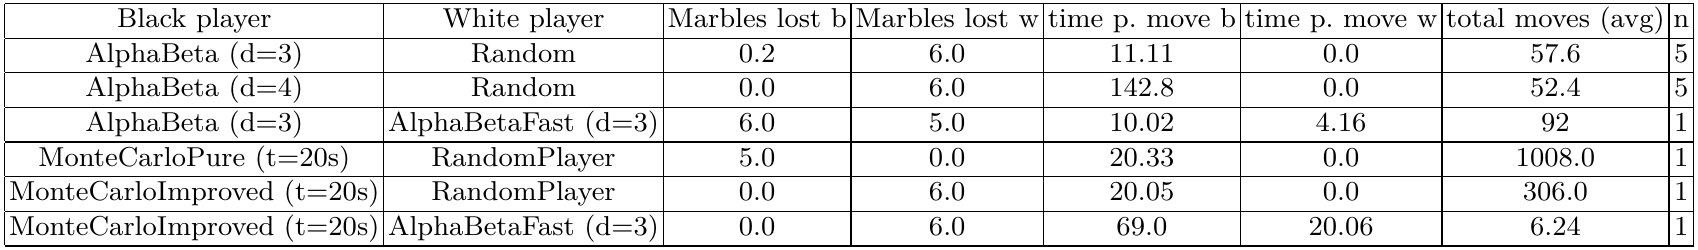
\includegraphics[width=12cm, keepaspectratio]{face_off_table.png}
		\end{figure}
	\end{adjustwidth}
\end{frame}

\begin{frame}
	\frametitle{Conclusion}
	\begin{itemize}
		\item Implementation simple, improvement requires a lot of engineering
		\item MCTS performed badly but with more time still promising
	\end{itemize}
\end{frame}
\end{document}